\documentclass{article}
\usepackage{tikz}
\usepackage{CJKutf8}
\usepackage{amsmath}
\usepackage{amsthm}
\begin{document}
\begin{CJK}{UTF8}{gbsn}
\newtheorem{Exercise}{习题}
\begin{Exercise}
  画出具有$3$个顶点的所有有向图(同构的只算一个)。
\end{Exercise}
\begin{Exercise}
  具有$p$个顶点的完全有向图中有多少条弧?
\end{Exercise}

\begin{Exercise}
  设$D$为一个有$p$个顶点$q$条弧的有向图。如果$D$为连通的,证明:$p-1\leq q \leq p(p-1)$。
\end{Exercise}
\begin{Exercise}
  设$D$为一个有$p$个顶点$q$条弧的强连通的有向图,则$q$至少是多大?
\end{Exercise}
\begin{Exercise}
  有向图$D$的图解如下图所示:
  
  \centering
  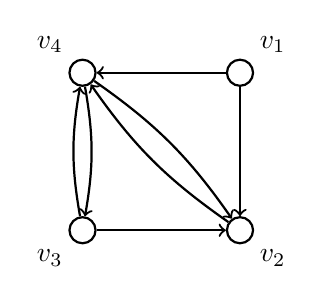
\begin{tikzpicture}[auto,
    specification/.style ={circle, draw, thick}]
   \node[specification] (A) [label=-135:$v_3$] at (0,0)  {};
   \node[specification] (B) [label=135:$v_4$] at (0,2)  {};
   \node[specification] (C) [label=45:$v_1$] at (2,2)  {};
   \node[specification] (D) [label=-45:$v_2$] at (2,0)  {};
   \draw[thick, ->] (A) to  (D);
   \draw[thick, ->] (C) to  (B);
   \draw[thick, ->] (C) to  (D);
   \draw[thick, ->] (A) to [bend left = 10] (B);
   \draw[thick, ->] (B) to [bend left = 10] (A);
   \draw[thick, ->] (B) to [bend left = 10] (D);
   \draw[thick, ->] (D) to [bend left = 10] (B);   
 \end{tikzpicture}\hspace{1cm}\\
 D

 \begin{enumerate}
  \renewcommand{\labelenumi}{(\theenumi)}
  \item 写出$D$的邻接矩阵及可达矩阵;
  \item 写出$D$的关联矩阵。
  \end{enumerate}
\end{Exercise}

\begin{Exercise}
  有向图$D$的图解如下图所示:

  \centering
  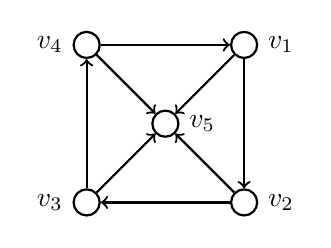
\begin{tikzpicture}[auto,
    specification/.style ={circle, draw, thick}]
   \node[specification] (A) [label=0:$v_1$] at (1,1)  {};
   \node[specification] (B) [label=0:$v_2$] at (1,-1)  {};
   \node[specification] (C) [label=180:$v_3$] at (-1,-1)  {};
   \node[specification] (D) [label=180:$v_4$] at (-1,1)  {};
   \node[specification] (E) [label=0:$v_5$] at (0,0)  {};
   
   \draw[thick, ->] (A) to  (B);
   \draw[thick, ->] (B) to  (C);
   \draw[thick, ->] (C) to  (D);
   \draw[thick, ->] (D) to  (A);
   \draw[thick, ->] (A) to  (E);
   \draw[thick, ->] (B) to  (E);
   \draw[thick, ->] (C) to  (E);
   \draw[thick, ->] (D) to  (E);   
 \end{tikzpicture}\hspace{1cm}\\
 D

求从顶点$v_2$到其余每个顶点的长$\leq 4$的所有有向通道的条数。 
\end{Exercise}
\begin{Exercise}
  设$T$为一棵正则$m$元有序树,它有$n_0$个叶子,$T$有多少条弧?
\end{Exercise}
\begin{Exercise}
  设$T$为一棵有$n_0$个叶子的二元树,出度为$2$的顶点数为$n_2$,试证$n_0=n_2+1$。
\end{Exercise}
\begin{Exercise}
  用数学归纳法证明每个比赛图中必有有向哈密顿路。
\end{Exercise}
\end{CJK}
\end{document}


%%% Local Variables:
%%% mode: latex
%%% TeX-master: t
%%% End:
